\chapter{General Concepts}

\section{Script}
At least one set of defined base elements or symbols,  is a requirement for all
writing systems. these symbols are individually termed as characters and
collectively called a script. simply  the set of the symbols required to
represent a writing system is called a script. a script may in turn be used to
represent more than one languages. Latin, Devanagari and Arabic are examples of
scripts. English, French, German, and Latin are all languages written using the
Latin script.

\section{Complex script }
\begin{wrapfigure}{r}{0.4\textwidth}
\begin{center}

\includegraphics[width=0.2\textwidth,height=0.2\textwidth,keepaspectratio]
{JanaSanskritSans_ddhrya.png}

{\tiny The Devanagari ddhrya-ligature, as displayed in the JanaSanskritSans
font.}
\end{center}
\end{wrapfigure}

Complex script is a writing system in which the shape or positioning of a
character
depends on its relation to other characters.

What makes it complex?
* Bi-directional: text is written right-to-left (For example: Arabic, Hebrew)
and left-to-right (For example: Devanagari)

* Context sensitive shaping and ligatures: Character may change shape depending
upon position.

* Ordering:
In Gujarati, Ki is where 'i' is place before 'K'.

//FIXME
What is a complex script? What makes it complex, some examples, screenshots
2-3 paragraph + images
How it differs from simple scripts like Latin Character

\section{Glyph }

A glyph is an element of writing. It can be a single character or a group of
characters.
Visually, if you see one or more characters form a single visual unit, it is
called a glyph.

In typography, it is "the specific shape, design, or representation of a
character".
\footnote{Ilene Strizver. "Confusing (and Frequently Misused) Type Terminology,
Part 1". fonts.com. Monotype Imaging.}

It is a particular graphical representation, in a particular typeface, of an
element of written language, which could be a grapheme, or part of a grapheme,
or sometimes several graphemes in combination.

To illustrate this concept, a set glyphs inside a Latin font (Fig.
\ref{Robotoglyph}) and a Malayalam font  (Fig. \ref{Meeraglyph}) as seen in
fontforge is given below.

\begin{figure}[h]
    \centering
    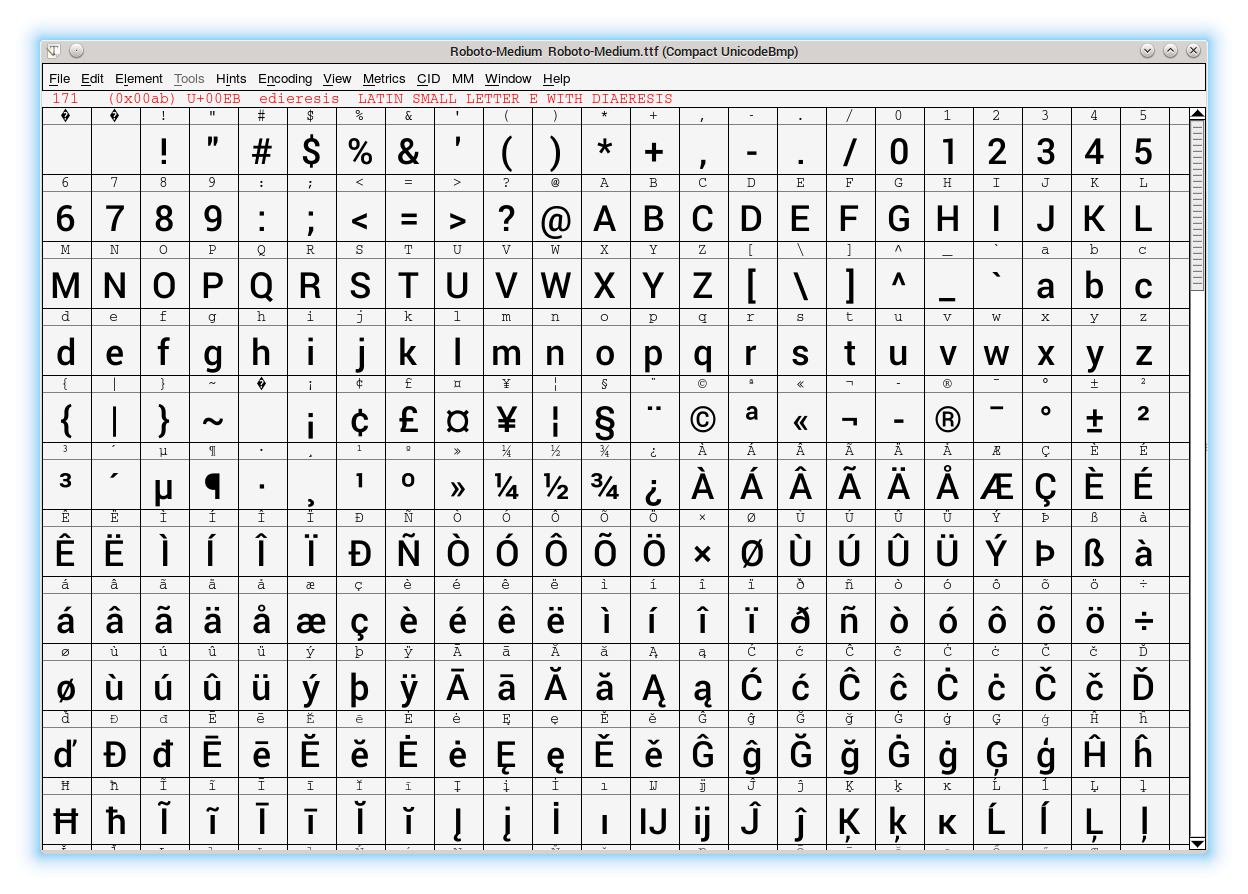
\includegraphics[width=0.8\textwidth]{glyph-fontforge-roboto.png}
    \caption{Glyphs inside Roboto font}
	\label{Robotoglyph}
\end{figure}

\begin{figure}[h]
    \centering
    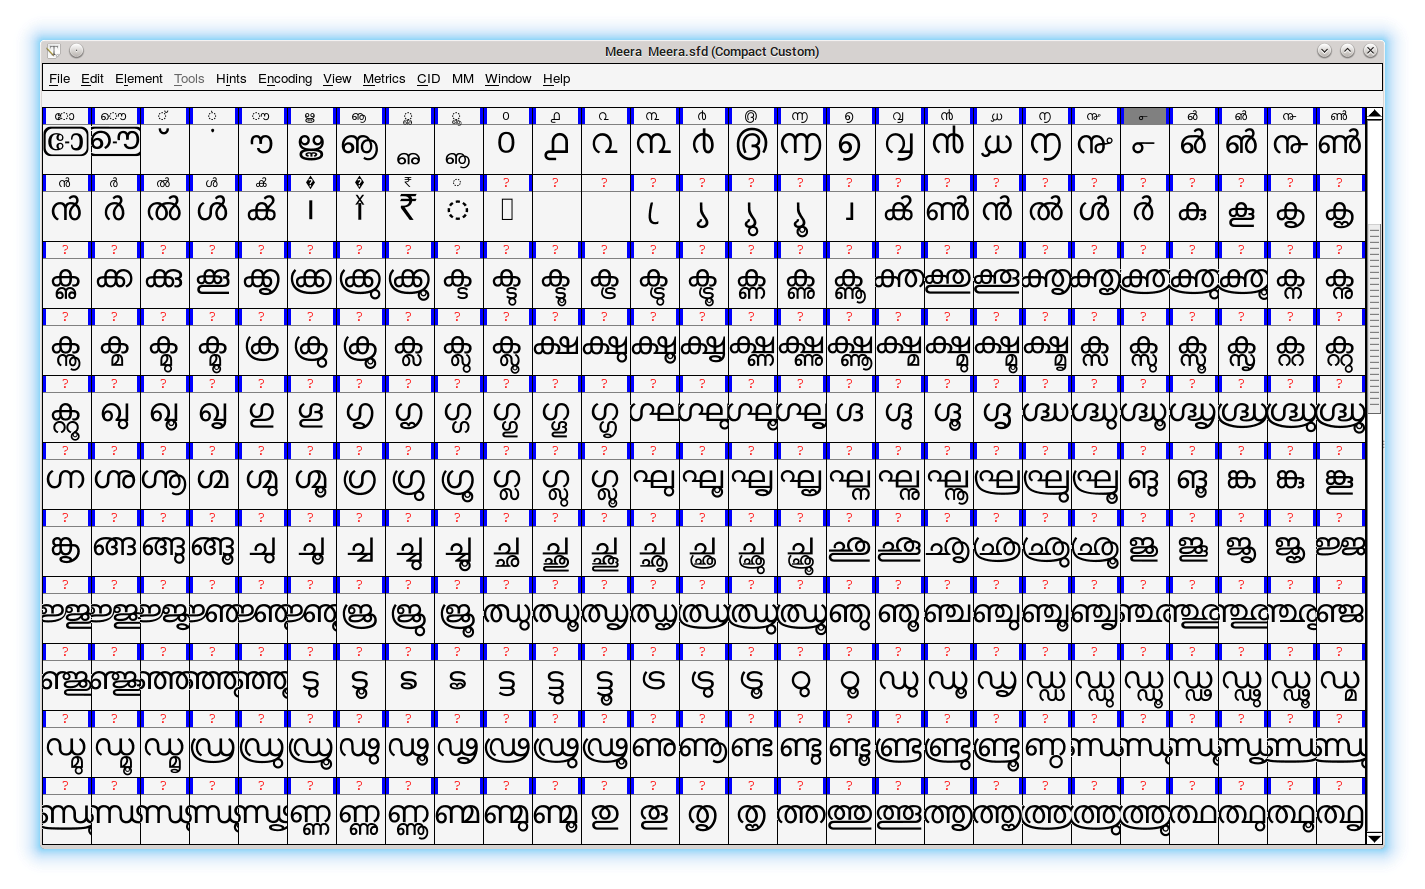
\includegraphics[width=0.8\textwidth]{glyph-fontforge-meera.png}
    \caption{Glyphs inside Meera font}
	\label{Meeraglyph}
\end{figure}

\begin{figure}[h]
    \centering
    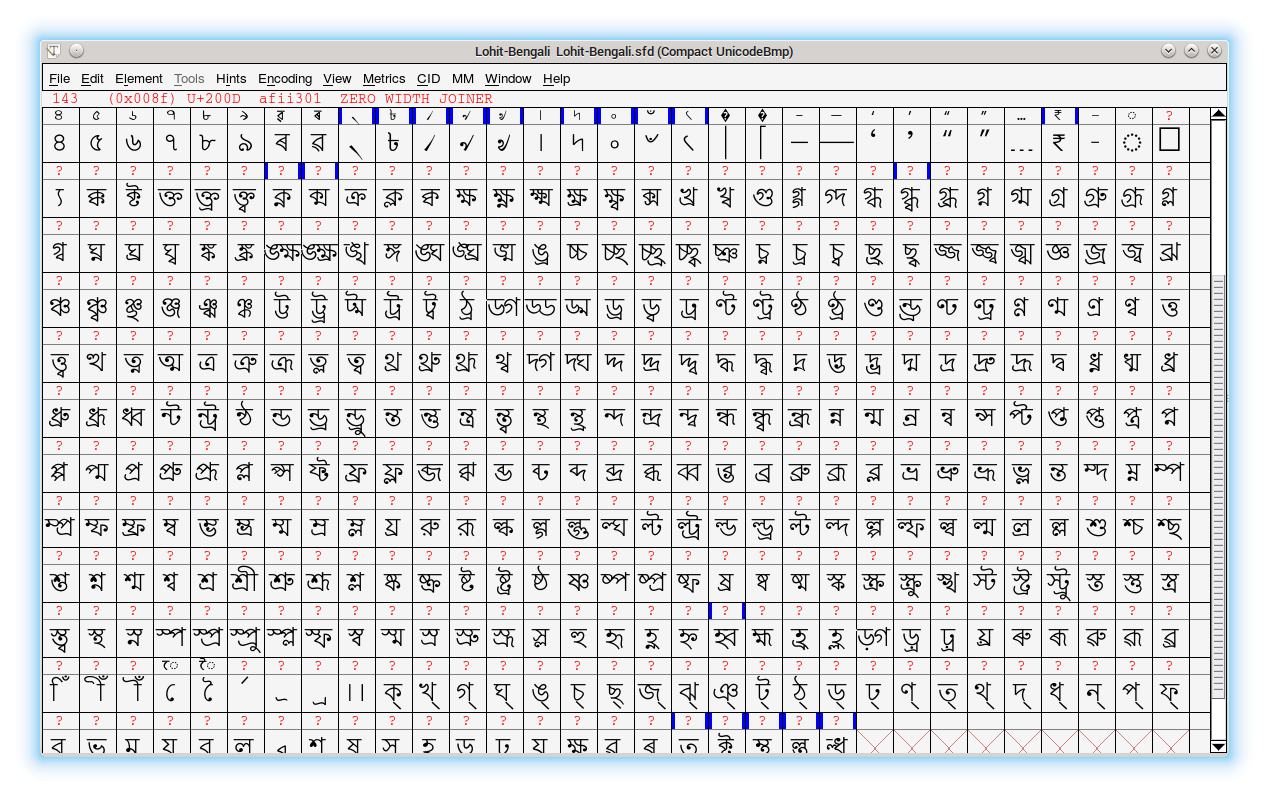
\includegraphics[width=0.8\textwidth]{glyph-fontforge-lohit-bengali.png}
    \caption{Glyphs inside Lohit Bengali font}
\end{figure}

\section{Ligatures }

In writing and typography, a ligature occurs where two or more graphemes or
letters are joined as a single glyph. Ligatures usually replace consecutive
characters sharing common components and are part of a more general class of
glyphs called "contextual forms", where the specific shape of a letter depends
on context such as surrounding letters or proximity to the end of a line.
\footnote{\url{https://en.wikipedia.org/wiki/Typographic_ligature}}

By way of example, the common ampersand '\&' represents the Latin conjunctive
word et, for which the English equivalent is the word "and". The ampersand's
symbol is a ligature, joining the old handwritten Latin letters e and t of the
word et, so that the word is represented as a single glyph.

The Brahmic abugidas make frequent use of ligatures in consonant clusters. The
number of ligatures employed may be language-dependent; thus many more ligatures
are conventionally used in Devanagari when writing Sanskrit than when writing
Hindi. Having 37 consonants in total, the total number of ligatures that can be
formed in Devanagari using only two letters is 1369, though few fonts are able
to render all of them.

\begin{figure}[h]
   \centering
   {\hindi\textexample द्ध्र्य }
   \caption{The Devanagari ddhrya-ligature {\hindi (द् + ध् + र् + य = द्ध्र्य)
} }
\end{figure}

\begin{figure}[h]
   \centering
   {\malayalam\textexample  ക്തു}
   \caption{The Malayalam kthu-ligature {\malayalam (ക + ് + ത + ു ) } }
\end{figure}

\begin{figure}[h]
  \centering
  {\gujarati\textexample સ +  ં = સં}
  \caption{The Gujarati 's' formed from SA and ANUSVARA}
\end{figure}

\section{Cluster/Syllable }

\section{Akhand }

\section{Ra Forms }
//FIXME
Explain Reph
Explain Rakar

\subsection*{Matra}
//FIXME
Explain prebase, postbase matra with examples and images

\section{Split Matra }

\section{Reordering }

\section{Zero Width Joiner }

\section{Zero Width Non Joiner }

\section{Stacking }

